\documentclass[]{beamer}
% Class options include: notes, notesonly, handout, trans,
%                        hidesubsections, shadesubsections,
%                        inrow, blue, red, grey, brown

% Theme for beamer presentation.
\usepackage{beamerthemesplit} 
% Other themes include: beamerthemebars, beamerthemelined, 
%                       beamerthemetree, beamerthemetreebars  
\newcommand{\der}{\text{d}}
\newcommand{\coder}[1]{\texttt{#1}}

\title{Fast simulation of advection equation using GPUs}    % Enter your title between curly braces
\author{Yair Daon}                 % Enter your name between curly braces
\institute{Courant Institute}      % Enter your institute name between curly braces
\date{\today}                    % Enter the date or \today between curly braces

\begin{document}

% Creates title page of slide show using above information
\begin{frame}
  \titlepage
\end{frame}
\note{Talk for 30 minutes} % Add notes to yourself that will be displayed when
                           % typeset with the notes or notesonly class options

\section{Problem Statement}
\begin{frame}
  \frametitle{Problem statement}   % Insert frame title between curly braces

  \begin{itemize}
  \item We'd like to simulate $\frac{\partial T}{\partial t} + \sum_{i=1}^{d} \frac{\partial u^{(i)}T}{\partial x^{(i)}} = 0$ 
  \item $T$ is a tracer - ``a drop of ink in water''.
  \item $d$ is the dimension. I'll show visualizations when $d=2$ and scaling results for $d=3$.
  \item Focus on flows such that $\sum_{i=1}^{d} \frac{\partial u^{(i)}}{\partial x^{(i)}} = 0$ - incompressible.
  \end{itemize}
\end{frame}
\note[enumerate]       % Add notes to yourself that will be displayed when
{                      % typeset with the notes or notesonly class options
\item Yair rocks.
\item It's true, he does!!!   
}



% Creates table of contents slide incorporating
% all \section and \subsection commands
%\begin{frame}
%  \tableofcontents
%\end{frame}


\section{Numerics}

\begin{frame}
  \frametitle{Numerical Method}   % Insert frame title between curly braces

  \begin{itemize}
  \item Use finite volume. Here's how we do it in 2D.
  \item Partition space to boxes. Denote centers by $(x_j, y_k)$. 
  \item Integrate the equation in all coordinates over box.
  \item Gives integrals that we estimate like $\int_{x_i - \frac{\Delta x}{2}}^{x_i + \frac{\Delta x}{2}} F(x,y_j) dx \approx F(x_i ,y_j)\Delta x$
  \item When the dust settlels, 
  $$
  \frac{\der T_{ij}}{\der t} = -\frac{uT(x_{i+\frac{1}{2}} , y_j) - uT(x_{i-\frac{1}{2}} , y_j)}{\Delta x} -\frac{vT(x_i , y_{j+\frac{1}{2}}) - vT(x_i , y_{j-\frac{1}{2}})}{\Delta y}.
  $$  
  \item $uT(x,y) = u(x,y) T(x,y)$ etc.
  \item Important - estimate $T$ on cell edges as an average of the two neighbouring cells.
  \item Result: an ODE of the form $\frac{\der T}{\der t} = AT$, with $A$ linear in $T$.
  \end{itemize}
\end{frame}

\begin{frame}
  \frametitle{Saving on memory access costs}   % Insert frame title between curly braces

  \begin{itemize}
\item Keep in mind, we want to simulate
  $$
  \frac{\der T_{ij}}{\der t} = -\frac{uT(x_{i+\frac{1}{2}} , y_j) - uT(x_{i-\frac{1}{2}} , y_j)}{\Delta x} -\frac{vT(x_i , y_{j+\frac{1}{2}}) - vT(x_i , y_{j-\frac{1}{2}})}{\Delta y}.
  $$  
  \item We'd like to use RK for $\frac{\der T}{\der t} = AT$. $A$ is just a convolution.
  \item Naive implementation has big cost of data transmission.
  \item We need $AT, A^2T, A^3T$ etc. locally on the GPU.
  \item Manually is nasty. Forming the matrix is a bad idea.
  \item Better - $T: \mathbb{N}^2 \to \mathbb{R}$ and $A:(\mathbb{N}^2 \to \mathbb{R}) \to (\mathbb{N}^2 \to \mathbb{R})$.  
  \item Mathematica can do this using $\lambda$ calculus.
  \item Bonus: switch RK method and dimension with zero effort.
  \end{itemize}
\end{frame}
\note{Speak clearly}  % Add notes to yourself that will be displayed when
                      % typeset with the notes or notesonly class options


\section{OpenCl Implementation}
\begin{frame}
  \frametitle{Python}   % Insert frame title between curly braces

  \begin{itemize}
  \item For the host side I used Andreas Kl\"ockner's PyOpenCl.
  \item Allows easy set up of OpenCl and data transfer.
  \item Relieves programmer from allocating and freeing data.
  \item Can create the kernel on the fly using python's string methods.
  \item Visualizations are also really easy, using matplotlib.
  \item For CUDA machines Andreas made PyCUDA.
  \item Incurs some overhead compared to C. I think it's worth it.
  \end{itemize}
\end{frame}
\note{Speak clearly}  % Add notes to yourself that will be displayed when
                      % typeset with the notes or notesonly class options

\begin{frame}
  \frametitle{Machines}   % Insert frame title between curly braces

  \begin{itemize}
  \item I ran the code on two CIMS boxes, opencl1 and opencl3. 
  \item Did the visualizations on my box. Speed tests on opencl3 using Cedar AMD GPU. 
  \end{itemize}
\end{frame}
\note{Speak clearly}  % Add notes to yourself that will be displayed when
                      % typeset with the notes or notesonly class options

\section{Results}
\begin{frame}
  \frametitle{Scaling}   % Insert frame title between curly braces
  \begin{columns}[c]
  \column{2in}  % slides are 3in high by 5in wide
  \begin{itemize}
  \item Observe weak scaling.
  \item RK3 kernel is big $\sim$ 80KB.
  \item RK2 kernel is $\sim$ 16KB.
  \item Rk3 accesses memory 3 times more than RK2.
  \item Advice: use \coder{time.time}.
  \end{itemize}
  \column{2in}
  \framebox{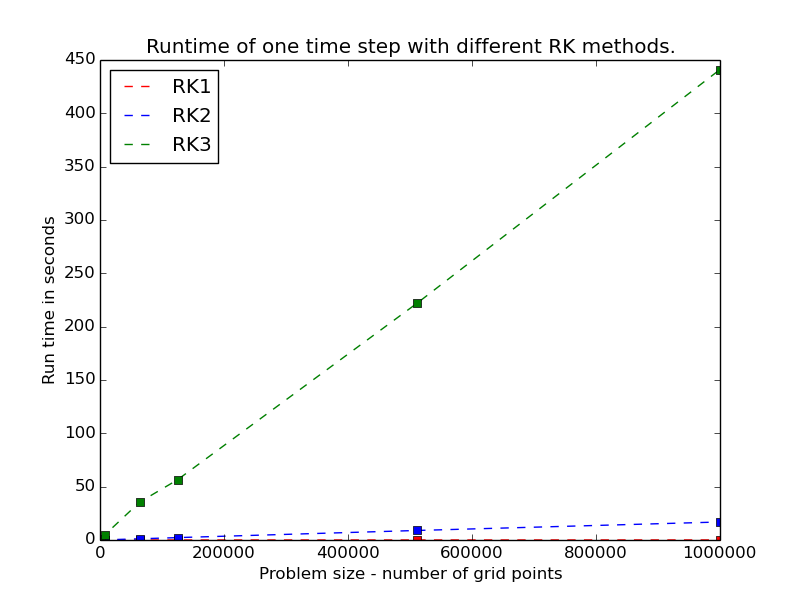
\includegraphics[height=2.0in , width = 2.0in]{pdf/3d.png}
  }
  \end{columns}
\end{frame}
\note{The end}       % Add notes to yourself that will be displayed when

\begin{frame}
  \frametitle{Visualization}   % Insert frame title between curly braces
  \begin{itemize}
  \item There's a short movie, if we have time.  
  \end{itemize}
\end{frame}
	

\section{Future}
\begin{frame}
  \frametitle{Now what?}   % Insert frame title between curly braces
 
  \begin{itemize}
  \item<1-> Take it to extreme scale - run on many GPUs using MPI.
  \item<2-> Nonlinear problems. $\lambda$ calculus may still be of use.
  \item<3-> Propagate uncertainties in time using openMP.
  \item<4-> Take a few time steps locally.
  \item<5-> Solve in one pass, for any fixed time (more suitable for CPUs).
  \item<6-> Adaptive meshes.
  \item<7-> Calculate approximate solution using dominant eigenvectors..
  \item<8-> Infer IC using deconvolution techiniques.
  \item<8-> Might be possible to use (parallel) Multigrid for that.
  \end{itemize}
\end{frame}
\note{The end}       % Add notes to yourself that will be displayed when

\end{document}